\documentclass[11pt,a4paper]{article}
\usepackage[spanish]{babel}
\usepackage[utf8]{inputenc}
\usepackage{amsmath, amssymb}
\usepackage{graphicx}
\usepackage{hyperref}
\usepackage{geometry}
\geometry{margin=2.5cm}

\title{\textbf{Diseño de un entorno de navegación urbana basado en grafos con waypoints para aprendizaje por refuerzo}}
\date{}

\begin{document}
\maketitle

\begin{abstract}
Se presenta el diseño e implementación de un entorno personalizado para \textit{Reinforcement Learning} (RL) denominado \texttt{WaypointNavigationEnv}, construido sobre \texttt{Gymnasium} y \texttt{NetworkX}. Este entorno modela un sistema de navegación sobre grafos dirigido a simular trayectorias urbanas con puntos intermedios (\textit{waypoints}), destino fijo, y control de penalizaciones por ciclos o acciones redundantes. La arquitectura permite escalar desde entornos pequeños hasta simulaciones urbanas amplias mediante técnicas de enmascaramiento de acciones, embeddings de nodos y métricas de progreso derivadas de caminos más cortos.
\end{abstract}

\section{Introducción}

En problemas de movilidad y planificación urbana, los agentes de aprendizaje por refuerzo deben operar en entornos donde las decisiones locales tienen consecuencias globales sobre tiempo, distancia y eficiencia del recorrido. Modelar estos escenarios requiere más que un simple grafo: se necesitan estructuras que integren representación espacial, restricciones topológicas y señales de recompensa que reflejen comportamiento inteligente.

El entorno \texttt{WaypointNavigationEnv} surge de esta necesidad. Se introduce una representación continua del espacio mediante \textit{embeddings nodales}, métricas de progreso basadas en Dijkstra y una arquitectura modular que permite extender el modelo a grafos reales obtenidos de redes urbanas (por ejemplo, OpenStreetMap).

\section{Analogía conceptual y dinámica de aprendizaje del algoritmo PPO}

El algoritmo \textit{Proximal Policy Optimization} (PPO) puede entenderse como un proceso de aprendizaje por refuerzo en el que el agente intenta mejorar su política de decisión sin dar pasos demasiado grandes que lo hagan “olvidar” lo que ya sabía.

Una forma natural de visualizarlo es imaginar un conductor aprendiendo a moverse por una ciudad compleja. Cada día repite su ruta, pero ajusta ligeramente su comportamiento: acelera un poco antes de una curva, toma una calle alternativa, o evita un embotellamiento que detectó previamente. PPO replica exactamente este comportamiento: experimenta, evalúa el resultado y ajusta la política solo dentro de una región controlada. 

Aplicado al entorno \texttt{WaypointNavigationEnv}, el agente PPO aprende patrones de navegación eficientes observando cómo sus acciones afectan el tiempo de viaje, el progreso hacia el destino y las penalizaciones por ciclos. En términos intuitivos, “aprende a conducir con propósito”, recordando lo que funciona y corrigiendo gradualmente lo que no, como un conductor que perfecciona su ruta diaria con experiencia acumulada.

\subsection{Reutilización de experiencias y generalización}

El algoritmo PPO no memoriza trayectorias exactas, sino que abstrae patrones de comportamiento a partir de múltiples recorridos. Cada episodio produce una secuencia de experiencias $(s_t, a_t, r_t, s_{t+1})$ que se almacenan en un buffer de \textit{rollouts}. Durante la fase de actualización, el agente estima las ventajas $\hat{A}_t$ para cada transición y ajusta su política global de modo que aumente la probabilidad de aquellas acciones que demostraron ser mejores de lo esperado.

De esta manera, las experiencias locales —por ejemplo, cómo aproximarse a un waypoint o evitar un ciclo en un barrio determinado— se transforman en conocimiento generalizable aplicable a otras zonas del grafo. El agente no recuerda posiciones específicas, sino \textit{principios de navegación}: cuándo avanzar, cuándo retroceder y cómo minimizar el costo de viaje. 

\subsection{Ejemplo en concreto}
Supongamos que el agente se encuentra en un cruce con tres caminos. Uno de ellos resulta más directo y requiere pasar por menos intersecciones. Tomar cualquiera de los otros implica atravesar más nodos, lo que se traduce en un mayor costo. A partir de esta experiencia, el agente aprende que, ante situaciones similares —aunque ocurran en distintos lugares o con pesos diferentes—, puede generalizar su comportamiento. Al normalizar los valores obtenidos, identifica un patrón que le indica cuál es la mejor decisión al enfrentarse a un cruce.

\begin{figure}[htbp]
  \centering
  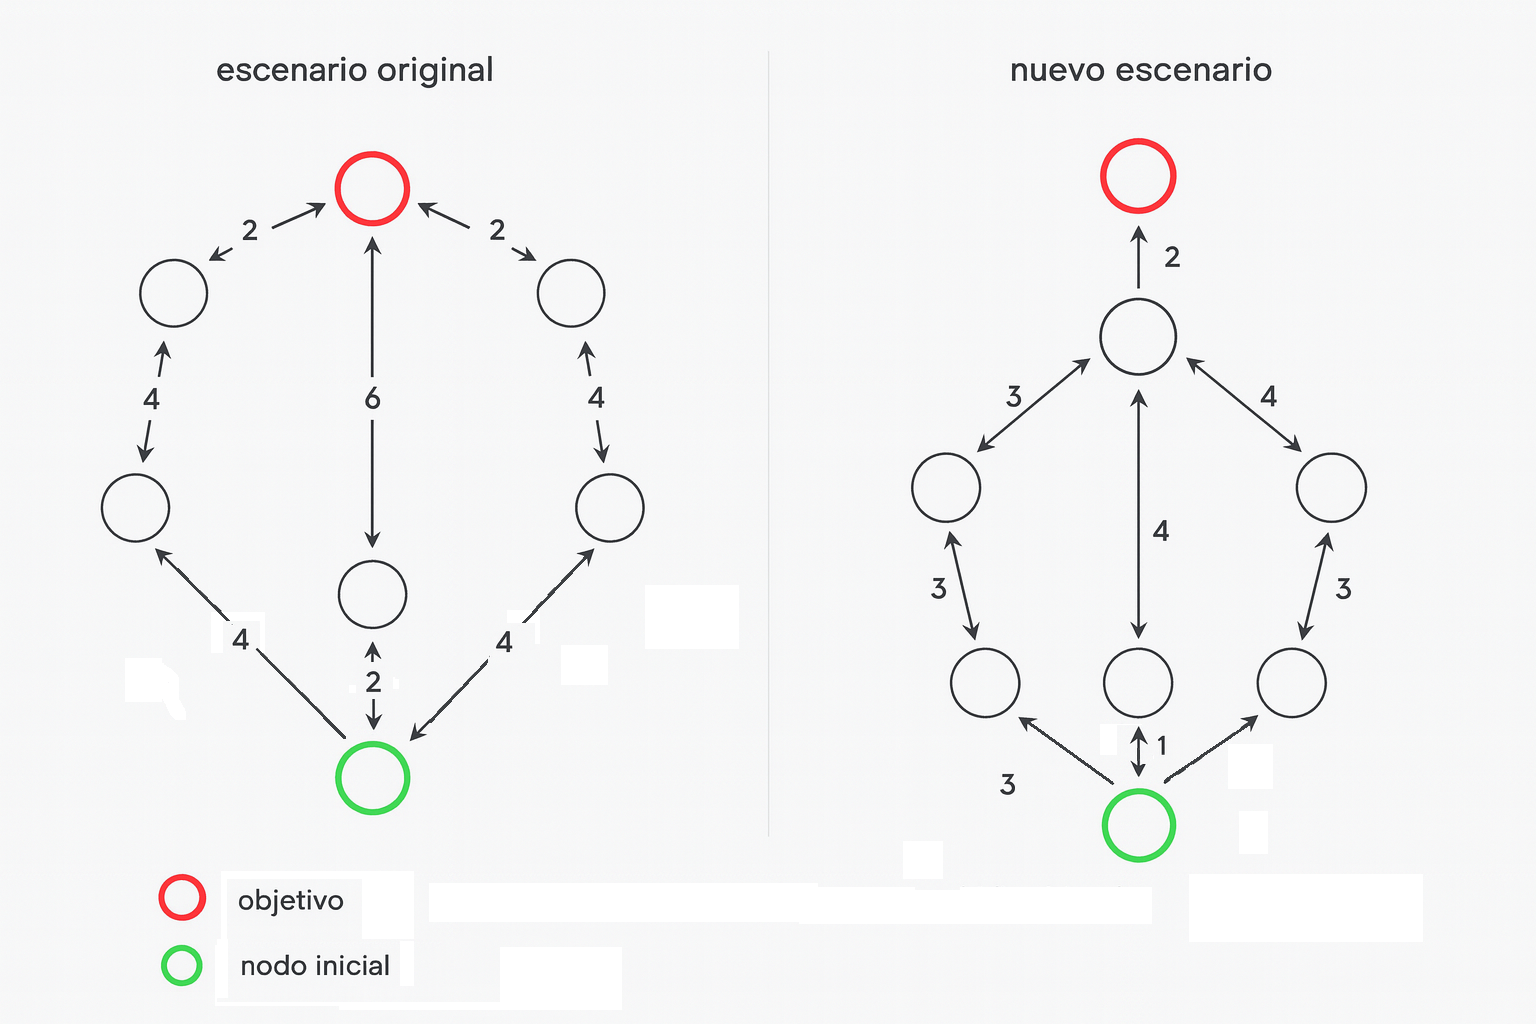
\includegraphics[width=.8\textwidth]{example.png}
  \caption{Agente en una situación real.}
  \label{fig:resultado}
\end{figure}

\section{Diseño del entorno}

El entorno base está construido sobre la clase \texttt{gym.Env} e implementa los métodos esenciales \texttt{reset()} y \texttt{step()}. Cada nodo del grafo se representa con un vector embebido que codifica información posicional o estructural. La observación entregada al agente combina tres componentes:

\begin{enumerate}
    \item El embedding del nodo actual.
    \item El embedding del siguiente waypoint y del destino.
    \item Escalares que representan distancia al destino, distancia al waypoint y fracción de pasos restantes.
\end{enumerate}

Esto da lugar a un vector continuo de observación de dimensión $3d + 3$, donde $d$ es la dimensión del embedding de cada nodo. Las acciones corresponden a la elección de un vecino válido del nodo actual, con un espacio discreto de tamaño máximo igual al grado más alto del grafo.

\subsection{Embeddings estructurales y métricas topológicas}

Cada nodo del grafo urbano se representa mediante un \textit{embedding} que combina tanto información espacial como estructural. Además de las coordenadas $(x, y)$ y el grado normalizado, se incorporan métricas de conectividad y centralidad que permiten capturar propiedades locales y globales del entorno. Estos atributos enriquecen la observación del agente y mejoran la capacidad del modelo para aprender patrones de navegación en zonas con distinta densidad vial.

\subsubsection{Conectividad avanzada}

\textbf{Grado de entrada (\textit{in\_degree})}: cantidad de calles que llegan a una intersección.  
\textit{Significado}: punto donde converge el tráfico.  
\textit{Ejemplo}: si llegan 4 calles $\rightarrow$ \texttt{in\_degree = 4}.

\textbf{Grado de salida (\textit{out\_degree})}: cantidad de calles que salen desde una intersección.  
\textit{Significado}: punto donde el tráfico se dispersa.  
\textit{Ejemplo}: si salen 4 calles $\rightarrow$ \texttt{out\_degree = 4}.

\textbf{Número de vecinos (\textit{neighbor\_count})}: cantidad de intersecciones conectadas directamente.  
\textit{Significado}: más vecinos implican más opciones de movimiento.  
\textit{Ejemplo}: nodo conectado con 4 intersecciones $\rightarrow$ \texttt{neighbor\_count = 4}.

\subsubsection{Análisis del vecindario}

\textbf{Grado promedio de vecinos (\textit{avg\_neighbor\_degree})}: promedio de conectividad de los vecinos.  
\textit{Significado}: si los vecinos están bien conectados, el nodo pertenece a una zona activa.  
\textit{Ejemplo}: grados [2, 4, 6, 8] $\rightarrow$ promedio = 5.

\textbf{Grado máximo de vecinos (\textit{max\_neighbor\_degree})}: el vecino más conectado.  
\textit{Significado}: tener un vecino con alta conectividad permite alcanzar muchas rutas.  
\textit{Ejemplo}: [2, 4, 6, 8] $\rightarrow$ máximo = 8.

\textbf{Grado mínimo de vecinos (\textit{min\_neighbor\_degree})}: el vecino menos conectado.  
\textit{Significado}: vecinos con pocas conexiones indican zonas más aisladas.  
\textit{Ejemplo}: [2, 4, 6, 8] $\rightarrow$ mínimo = 2.

\textbf{Desviación estándar del grado de vecinos (\textit{neighbor\_degree\_std})}: mide la variabilidad entre los grados de los vecinos.  
\textit{Significado}: alta variabilidad indica zonas de transición (por ejemplo, entre barrios).  
\textit{Ejemplo}: [2, 2, 8, 8] $\rightarrow$ \texttt{std = 3.0}.  
Esta medida es útil porque en zonas de transición la elección del camino tiene más impacto que en zonas céntricas, donde las decisiones pueden simplificarse sin pérdida de rendimiento.

\subsubsection{Medidas de centralidad}

\textbf{Centralidad de grado (\textit{degree\_centrality})}: cuantifica la importancia estructural de un nodo dentro de la red.  
\textit{Fórmula}: $\texttt{degree} / (\texttt{total\_nodos} - 1)$  
\textit{Significado}: mide la relevancia topológica local de una intersección dentro del grafo urbano.

\textbf{Centralidad de intermediación aproximada (\textit{betweenness\_approx})}: estima si un nodo actúa como puente entre distintas zonas de la red.  
\textit{Fórmula simplificada}: $\texttt{neighbor\_count} / \texttt{total\_nodos}$ (aproximación local).  
\textit{Significado}: refleja qué tan probable es que el tráfico pase por ese nodo al conectar diferentes sectores.

\subsubsection{Vector final de embedding}

El embedding final de cada nodo $v_i$ se construye concatenando todos estos atributos normalizados:

\[
E(v_i) = [x_i, y_i, \texttt{in\_degree}, \texttt{out\_degree}, \texttt{neighbor\_count}, \texttt{avg\_neighbor\_degree}, \texttt{max\_neighbor\_degree}, \texttt{min\_neighbor\_degree}, \texttt{neighbor\_degree\_std}, \texttt{degree\_centrality}, \texttt{betweenness\_approx}]
\]

Esta representación multidimensional permite al agente de RL aprender no solo a moverse, sino a razonar sobre la estructura de la ciudad, diferenciando zonas densas, periféricas y de transición.

\section{Wrapper de enmascaramiento de acciones}

El entorno se complementa con un \texttt{ActionMaskingWrapper}, encargado de filtrar acciones inválidas o redundantes. Este módulo implementa:
\begin{enumerate}
    \item \textbf{Máscaras de acción dinámicas:} solo las acciones que conducen a vecinos válidos y productivos (más cercanos al objetivo) son habilitadas.
    \item \textbf{Prevención de ciclos:} el wrapper mantiene una cola de los últimos nodos visitados y un contador de visitas, aplicando penalizaciones progresivas o truncando el episodio ante la detección de bucles.
    \item \textbf{Selección de respaldo:} si todas las acciones son inválidas, el wrapper elige una acción de respaldo que mantenga la continuidad del episodio.
\end{enumerate}

\section{Aplicaciones y escalabilidad}

El entorno está diseñado para escalar desde redes sintéticas hasta ciudades reales. En un grafo urbano con miles de nodos, las distancias se calculan mediante Dijkstra ponderado, aunque para entornos de gran escala se recomienda:
\begin{itemize}
    \item Precomputar distancias entre puntos relevantes y almacenarlas en caché.
    \item Usar heurísticas A* para aproximar distancias.
\end{itemize}

\section{Naturaleza discreta del entorno}

El entorno \texttt{WaypointNavigationEnv} es de naturaleza \textbf{discreta} tanto en su espacio de acciones como en su evolución temporal. Cada paso (\texttt{step}) representa una transición entre nodos de un grafo dirigido o no dirigido, donde las acciones disponibles corresponden al conjunto finito de vecinos del nodo actual. 

Esto implica que el agente no se mueve en un espacio continuo, sino a través de \textit{estados discretos} representados por identificadores de nodos. Cada acción seleccionada se traduce en un desplazamiento atómico a un nodo adyacente, seguido por una evaluación de recompensa. De esta forma, la dinámica del entorno sigue el modelo clásico de procesos de decisión de Markov (MDP) con estado discreto \( s_t \in S \) y acción discreta \( a_t \in A(s_t) \).

A pesar de esta discretización topológica, las observaciones entregadas al agente pueden incluir componentes continuas (como los embeddings de nodos o las distancias ponderadas), lo que genera un entorno \textit{mixto}: discreto en estructura, continuo en representación.

\section{Conclusión}

El entorno \texttt{WaypointNavigationEnv} constituye una plataforma flexible y extensible para estudiar navegación basada en grafos dentro del marco del aprendizaje por refuerzo. Su diseño modular, junto con el wrapper de control de acciones y los embeddings estructurales, permite modelar comportamientos realistas de agentes en entornos complejos, equilibrando fidelidad y eficiencia computacional. 

En síntesis, este trabajo traduce el concepto abstracto de moverse en un grafo a un escenario urbano verosímil, en el que el agente no solo aprende a moverse, sino a \textit{navegar con propósito}.

\bibliographystyle{plain}
\begin{thebibliography}{9}
\bibitem{gymnasium} Farama Foundation. \textit{Gymnasium: A Toolkit for Reinforcement Learning}. Disponible en: \url{https://gymnasium.farama.org}
\bibitem{networkx} Hagberg, A. A., Schult, D. A., y Swart, P. J. (2008). \textit{Exploring network structure, dynamics, and function using NetworkX}. In Proceedings of the 7th Python in Science Conference (SciPy2008).
\bibitem{rlbook} Sutton, R. S., y Barto, A. G. (2018). \textit{Reinforcement Learning: An Introduction}. MIT Press.
\end{thebibliography}

\end{document}
